\documentclass[usenames,table,dvipsnames,aspectratio=169]{beamer}
\usepackage[utf8]{inputenc}
\usepackage[spanish]{babel}
\usepackage{beamerthemeshadow}
\usepackage{times}
\usepackage{graphicx}
\usepackage{amsmath,amssymb,amsfonts,latexsym,stmaryrd}
\usepackage{tabularx}
\usepackage{colortbl}
\usepackage{tikz}
\usepackage{xcolor}
\usepackage{mdwlist}
\usepackage{fancybox}
\usepackage{setspace}
\usepackage{courier}
\usepackage{hyperref}
\usepackage{beamerthemeshadow}
\usepackage{shadow}
\usepackage{listings}
\usepackage{mdwlist}
\usepackage{multicol}
\usepackage{ragged2e} % para justificar texto
\usepackage{textcomp} % Para usar simbolos en texto tipo +- etc
\usepackage[binary-units]{siunitx}
\usepackage[absolute,overlay]{textpos}
  \setlength{\TPHorizModule}{1mm}
  \setlength{\TPVertModule}{1mm}
\usepackage{pbox}
\usepackage{scrextend}
\usepackage{tikzsymbols}
\usepackage{verbatim}
\usepackage{beamerthemesplit}
\usepackage[most]{tcolorbox}
\usepackage{cite}

\usetikzlibrary{fit,positioning}
\usetikzlibrary{calc}
\pgfdeclarelayer{background}
\pgfdeclarelayer{foreground}
\pgfsetlayers{background,main,foreground}
\usetheme{default}

\definecolor{OliveGreen}{RGB}{2,80,1}
\definecolor{LigthOrange}{RGB}{255,255,200}
\definecolor{gray97}{gray}{.97}
\definecolor{Gray}{RGB}{171,174,178}

\definecolor{ShadowColor}{RGB}{130,150,190}

%%%%%%%%%%%%%%%%%%%%%%%%%%%%%%%%%%%%%%%%%%%%%%%%%%%%%%%%%%%%%%%%%%%%%%%%%%%%%%%%%%%%%%%%
%Para hacer cajas de texto con sombras lindas
\makeatletter
\newcommand\Cshadowbox{\VerbBox\@Cshadowbox}
\def\@Cshadowbox#1{%
  \setbox\@fancybox\hbox{\fbox{#1}}%
  \leavevmode\vbox{%
    \offinterlineskip
    \dimen@=\shadowsize
    \advance\dimen@ .5\fboxrule
    \hbox{\copy\@fancybox\kern.5\fboxrule\lower\shadowsize\hbox{%
      \color{ShadowColor}\vrule \@height\ht\@fancybox \@depth\dp\@fancybox \@width\dimen@}}%
    \vskip\dimexpr-\dimen@+0.5\fboxrule\relax
    \moveright\shadowsize\vbox{%
      \color{ShadowColor}\hrule \@width\wd\@fancybox \@height\dimen@}}}
\makeatother
%%%%%%%%%%%%%%%%%%%%%%%%%%%%%%%%%%%%%%%%%%%%%%%%%%%%%%%%%%%%%%%%%%%%%%%%%%%%%%%%%%%%%%%%%%%%

\graphicspath{
{../img/}
}

\mode<presentation>{
	\usetheme{Copenhagen}
	\useoutertheme{infolines}
}

\setbeamercovered{invisible}


\title{Sistemas de Numeración}
\subtitle{Representación de números reales}


\author{Alejandro Furfaro}
\date{\today}

\begin{document}

\begin{frame}[plain]{Representación de números reales}
 \begin{figure}[ht!]
  \centering 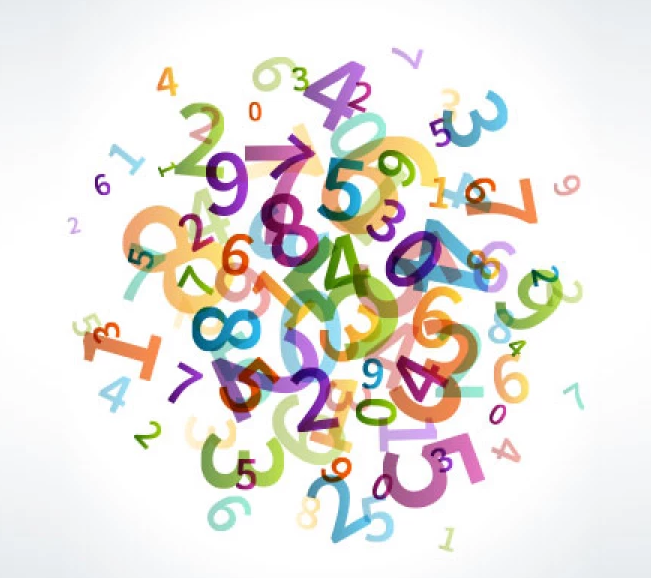
\includegraphics [width =0.25 \textwidth ]{Numbers.png}
 \end{figure}
 \vspace{-1cm}
 \titlepage
\end{frame}

\begin{frame}{Temario}
 \begin{textblock*}{\textwidth}(0.4cm,1.5cm)
  \footnotesize
  \tableofcontents
 \end{textblock*}
\end{frame}

\AtBeginSubsection[]
{
\begin{frame}{Temario}
 \begin{textblock*}{\textwidth}(0.4cm,1.5cm)
  \setcounter{tocdepth}{2}
  \tableofcontents[currentsection, currentsubsection, sectionstyle=show/shaded, subsectionstyle=show/shaded]
 \end{textblock*}
\end{frame}
}

\section{Números Reales}
\subsection{Representación digital del mundo real}
\begin{frame}{Números Reales}
 \begin{textblock*}{.5\textwidth}(0.4cm,1.2cm)
  \begin{itemize}[<+(1)->]\justifying  \parskip 0.2cm
   \item El rango de los números reales comprende desde $-\infty$ hasta $+\infty$.
   \item Los registros de un procesador tienen resolución finita.
   \item Por lo tanto un computador solo puede representar un sub conjunto de $\Re$.
   \item Además, no es solo un tema de magnitud sino de resolución.
  \end{itemize}
 \end{textblock*}
 \only<6->{
  \begin{textblock*}{.5\textwidth}((0.4cm+0.5\textwidth),1.2cm)
   \centering 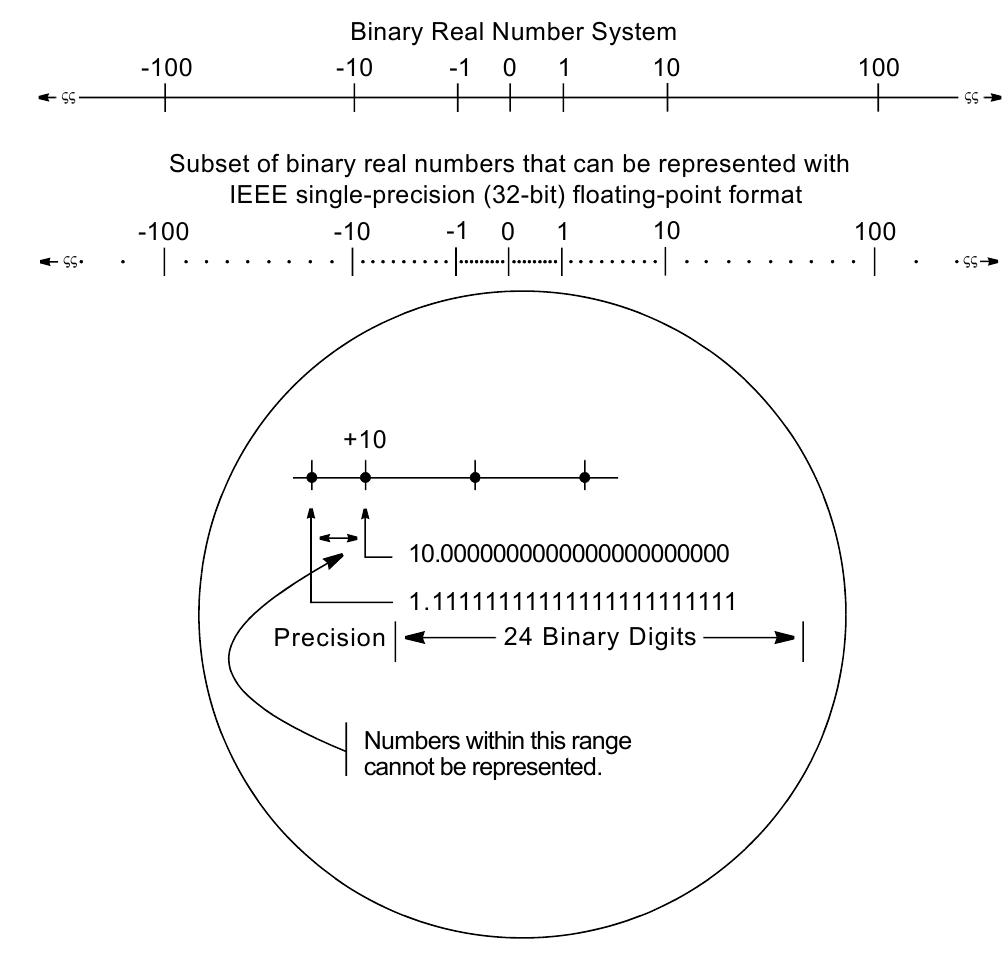
\includegraphics[width=\textwidth]{NumerosRealesenBinario.png}
  \end{textblock*}
 }
\end{frame}

% \subsection{Introducción}
\begin{frame}{Representación de Números Reales}
 \begin{textblock*}{\textwidth}(0.2cm,1.2cm)
  \begin{itemize} [<+(1)->]\justifying
   \item Un computador necesita soportar operaciones con números fraccionarios, denominados  en matemática como Números Reales.
   \item Ejemplos:
  \end{itemize}
 \end{textblock*}
 \begin{textblock*}{\textwidth}(0.9cm,3cm)
   \only<4->{$\pi=3.14159265358979323846..._{10}$\\}
   \only<5->{$e=2.7182818284590452353602874713527..._{10}$\\}
   \only<6->{$0.000000001_{10}$, ó $1.0_{10} x 10^{9}$ (nano metros por ejemplo)\\}
   \only<7->{$3,155,760,000$, ó $3.15576_{10} x 10^{9} $ segundos en un siglo\\}
 \end{textblock*}
 \begin{textblock*}{\textwidth}(0.2cm,4.9cm)
  \begin{itemize} [<+(5)->]\justifying
   \item En los tres primeros ejemplos se trata de números fraccionarios pequeños
   \item Pero el último es un número entero, pero tan grande que no puede ser representado mediante una variable entera de \SI{32}{\bit}
   \item En el tercer número se emplea \textbf{\textit{notación científica}}.
   \item En particular, cuando solo tiene un dígito no nulo como parte entera, y el resto se desplazan hacia la parte fraccionaria, ajustando el exponente, se habla de \textbf{\textit{Notación Científica Normalizada.}}
  \end{itemize}
 \end{textblock*}
\end{frame}

\begin{frame}{Notación Científica}
 \begin{textblock*}{\textwidth}(0.4cm,1.2cm)
  \begin{itemize}[<+->] \justifying
   \item Para el caso de los números reales se trabaja en \textbf{\textit{\color{blue}    notación científica}}.\\
   \begin{center}  \shadowbox{ $n= \pm f*10^e$ } \end{center}
   \item  $-725.832 = -7.25832*10^{2} = -725.832*10^{0}$
   \item  $3.14 = 0.314*10^{1} = 3.14*10^{0}$
   \item  $0.000001 = 0.1*10^{-5} = 1.0*10^{-6}$
   \item  $1941 = 0.1941*10^{4} = 1.941*10^{3}$
   \item Para unificar la representación  se recurre a la \textbf{\textit{\color{blue}notación científica normalizada}} \color{black}, en donde:\\
%   \vspace{0.3cm}
   \begin{center}
    $1 \leq$ \textbf{\textit{\color{blue}f}} \color{black} $<$ 9 ,y \textbf{\textit{\color{blue}e}} \color{black} es un entero con signo.
   \end{center}
  \end{itemize}
 \end{textblock*}
\end{frame}

\begin{frame}[t]{Notación Científica en el sistema Binario}
 \begin{textblock*}{\textwidth}(0.4cm,1.2cm)
  \begin{itemize} \justifying
   \item En el sistema binario la expresión de un número en notación científica normalizada es:\\
    \begin{center} \shadowbox{ $n= \pm f*2^e$  } \end{center}
   \vspace{0.3cm}
   \item En donde:\\
   \vspace{0.3cm}
   \begin{center}
 $0.5 \leq$ \textbf{\textit{\color{blue}f}} \color{black} $<$ 1 , 
y \textbf{\textit{\color{blue}e}} \color{black} es un entero con signo.
   \end{center}
  \end{itemize}
 \end{textblock*}
\end{frame}

\begin{frame}{Formatos de representación en un computador}
 \begin{textblock*}{\textwidth}(0.2cm,1.2cm)
  \begin{itemize} [<+(1)->]\justifying
   \item Al trabajar con números reales en un computador, enfrentamos un problema de primer magnitud: redondear cifras en una cantidad de bits acotada.
   \item Existen dos formatos de representación para número reales en un computador:
   \begin{itemize}
    \item Punto fijo
    \item Punto flotante
   \end{itemize}
   \item En general se impone la representación en punto flotante, dado que su rango de números representables con la misma cantidad de bits, es muchísimo mas amplio.
   \item La representación en Punto fijo permite utilizar los mismos registros de propósito general y la misma aritmética que se emplea con números enteros. La posición del punto decimal queda fija, por lo cual los resultados de las operaciones básicas son los mismos que para números enteros.
   \item Punto fijo es práctico en cálculos de rango numérico acotado. Ej: temperatura, presión, humedad, y demás magnitudes físicas cuyo rango es de algunos centenares de unidades a lo sumo, y requerimientos de precisión moderados.
  \end{itemize}
 \end{textblock*}
\end{frame}

\begin{frame}{Representación binaria en Punto Fijo con signo}
 \begin{textblock*}{\textwidth}(0.2cm,1.2cm)
  \begin{itemize}[<+(1)->]  \justifying \parskip 0.3cm
   \item Se representan mediante una expresión del tipo:\\
   $\color{blue}(a_{n}a_{n-1}\dots a_0.a_{-1}a_{-2}\dots a_{-m})_{2} = (-1)^{s}*(a_{n}*2^{n}+\dots + a_{0}*2^{0} + a_{-1}*2^{-1} + a_{-2}*2^{-2} +\dots+ a_{-m}*2^{-m})$
   \item Donde:
   \begin{itemize} \justifying
    \item \textbf{\textit{\color{blue}s}} \color{black}es el signo: \textbf{0} si el número es positivo y \textbf{1} si es negativo
    \item \textbf{\textit{\color{blue}$a_i$}} $\in  \mathbb{Z} $ y  $0 \leq$ \textbf{\textit{\color{blue}$a_i$}} $\leq 1$, $\forall$ \textbf{\textit{\color{blue}i}}\color{black} \textit{= -m, -1, 0, 1,\dots n}
   \end{itemize}
   \item Distancia entre dos números consecutivos es $2^{-m}$.
   \item \color{red}\textit{Deja de ser un rango continuo de números para transformarse en un rango discreto.}
  \end{itemize}
 \end{textblock*}
\end{frame}

\begin{frame}{Punto Flotante: Motivación}
 \begin{textblock*}{\textwidth}(0.2cm,1.2cm)
  \begin{itemize} [<+(1)->]\justifying
   \item Existe un rango amplio de aplicaciones que trabajan con números reales, y que además plantean requisitos muy estrictos de precisión.
   \item Para éstas resulta mucho mas adecuado el uso de punto flotante.
   \item Está basado en notación científica.
   \item En punto flotante un número se representa mediante un entero \textit{con signo} y de precisión fija llamado \textit{significando} o \textit{mantisa}, el que es escalado por otro entero también \textit{con signo} que se emplea como \textit{exponente} de una \textit{base} numérica fija.
   \item De este modo, cualquier número real puede ser representado en notación científica por medio de la siguiente expresión:
  \end{itemize}
  \only<6->{
   \begin{equation}\label{eq:scinot}
     n = m * b^e
   \end{equation}
   }
{\hangindent=0.8cm
\hangafter=1
\only<7->{\justifying donde \textit{m} representa la \textit{mantisa}, \textit{b} la \textit{base} numérica de representación, y \textit{e} el \textit{exponente} al que debe ser elevada la base.
}
\par}
 \end{textblock*}
\end{frame}

\begin{frame}{Punto Flotante: Precisión, Rango, Normalización}
 \begin{textblock*}{\textwidth}(0.2cm,1.2cm)
  \begin{itemize} [<+(1)->]\justifying
   \item La cantidad de bits de la \textit{mantisa} se relaciona con la precisión que puede obtenerse al representar un número irracional.
   \item Un número de precisión \textit{p} es aquel cuya representación emplea \textit{p} bits para la \textit{mantisa}, donde \textit{p} incluye el dígito correspondiente a su parte entera.
   \item El \textit{exponente}, por su parte, establece el rango de números que puede representarse.
   \item La expresión (1), sugiere que cada número puede tener tantas representaciones como combinaciones posibles existan entre los valores de \textit{exponente} y \textit{mantisa}.
   \item Para evitar tales ambig\"{u}edades, se recurre a una representación normalizada en que la \textit{mantisa} tiene un solo dígito entero. En \textit{base} 2, la simplificación evidente: hay solo dos valores posibles: $0$ o $1$.
   \item Si se asume que el dígito entero de la \textit{mantisa} siempre vale 1, se evita su inclusión.
   \item Se suma así a la \textit{mantisa} un bit adicional optimizando la precisión del número.
   \item Esta notación se denomina notación punto flotante normalizada.
  \end{itemize}
 \end{textblock*}
\end{frame}

\begin{frame}{Punto Flotante: Precisión, Rango, Normalización}
 \begin{textblock*}{\textwidth}(0.2cm,1.2cm)
  \begin{itemize} [<+(1)->]\justifying
   \item Un número real de precisión \textit{p} en base 2 puede expresarse de acuerdo con la siguiente expresión:\\
   \centering $n = \pm(1.m_{1}m_{2}m_{3}\dots m_{(p-2)}m_{(p-1)}) * 2^e$
   \item En su versión polinómica:\\
   \centering $n = \pm 1 + m_{1}\cdot 2^{-1} +  m_{2}\cdot 2^{-2} + \dot  m_{(p-1)}\cdot 2^{-(p-1)}$
   \item Esto sugiere que si aumentando la cantidad de bits del \textit{significando}, aumenta la precisión \textit{p}.
   \item Para una precisión \textit{p} dada, solo se puede representar un subconjunto de valores discretos pertenecientes a $\mathbb{R}$. Nunca al conjunto completo.
   \item En el siguiente slide representamos el conjunto discreto de Números Reales que pueden representarse para una dada Precisión \textit{p}.
   \item Puede verse que entre dos números consecutivos existe un intervalo de números reales que no pueden ser representados con esta Precisión ya que su \textit{mantisa} requiere más bits que la cantidad establecida por \textit{p}.
  \end{itemize}
 \end{textblock*}
\end{frame}

\begin{frame}{Punto Flotante: Precisión, Rango, Normalización}
 \begin{textblock*}{\textwidth}(0.2cm,1.2cm)
  \centering 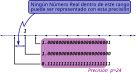
\includegraphics[width=.9\textwidth]{RealNumbers-1.pdf}
 \end{textblock*}
\end{frame}

\subsection{Normalización}
\begin{frame}{Situación inicial}
 \begin{textblock*}{\textwidth}(0.2cm,1.2cm)
  \begin{itemize} [<+->]\justifying \parskip .15cm
   \item Durante los años 60 y 70 cada fabricante de hardware que incluyó Unidades de Punto Flotante en la CPU de sus computadores optó por criterios de diseño particulares, en lo referente a la representación de los números.
   \item La cantidad de bits para \textit{mantisa}, \textit{exponente}, y la representación de cada uno de estos valores respecto del signo, así como los criterios para el redondeo en las operaciones, entre otros aspectos variaban de un procesador a otro.
   \item La precisión inherente de cada máquina era diferente, y por consecuencia, al ir acumulando resultados intermedios redondeados mediante criterios diferentes (truncado vs redondeo al mas próximo, por ejemplo), generaban resultados finales sensiblemente diferentes para un mismo algoritmo de cálculo (en rigor para algoritmos idénticos).
   \item Esta situación no resulta aceptable.
  \end{itemize}
 \end{textblock*}
\end{frame}

\begin{frame}{Situación inicial}
 \begin{textblock*}{\textwidth}(0.2cm,1.2cm)
  \begin{itemize} [<+->]\justifying \parskip .15cm
   \item Para solucionar esta divergencia se recurrió a una normalización del formato de representación de números en Punto Flotante.
   \item En 1985 se publica la primer especificación de una norma internacional a cargo del IEEE conocida como IEEE-754.
   \item Establece los formatos y criterios de cálculo para poner en común no solo el formato de representación, sino además otros aspectos relativos a las operaciones con estos números, tales como los criterios de redondeo, eventuales excepciones ante situaciones de borde como overflow, denormalización, etc.
   \item Por entonces, en 1985, la unidad de punto flotante que mas se había comercializado por lejos era el diseño de Intel de su Co Procesador de Punto Flotante 8087, presentado en 1978 junto al procesador 8086 y 8088 que IBM seleccionaría para su primer computador personal (IBM PC). Por tal motivo buena parte de la especificación IEEE-754 de 1985 ha tenido una marcada influencia de éste diseño.
  \end{itemize}
 \end{textblock*}
\end{frame}

\begin{frame}[t]{Formatos IEEE 754}
 \begin{textblock*}{\textwidth}(0.4cm,1.5cm)
  \only<1->{\includegraphics[width=\textwidth]{IEEE-754-layer1.pdf}}
 \end{textblock*} 
 \begin{textblock*}{\textwidth}(0.4cm,1.5cm)
  \only<2->{\includegraphics[width=\textwidth]{IEEE-754-layer2.pdf}}
 \end{textblock*} 
 \begin{textblock*}{\textwidth}(0.4cm,1.5cm)
  \only<3->{\includegraphics[width=\textwidth]{IEEE-754-layer3.pdf}}
 \end{textblock*} 
 \begin{textblock*}{\textwidth}(0.4cm,1.5cm)
  \only<4->{\includegraphics[width=\textwidth]{IEEE-754-layer4.pdf}}
 \end{textblock*} 
 \begin{textblock*}{\textwidth}(0.4cm,1.5cm)
  \only<5->{\includegraphics[width=\textwidth]{IEEE-754-layer5.pdf}}
 \end{textblock*} 
\end{frame}

\begin{frame}{IEEE-754}
 \begin{textblock*}{\textwidth}(0cm,1.2cm)
  \begin{itemize} [<+->]\justifying \parskip .12cm
   \item Cada formato consta finalmente de dos números de punto fijo: el \textit{significando}, y el \textit{exponente}. Ambos números signados.
   \item De acuerdo con la cantidad de bits de éstos, los números reales representables tienen diferentes precisiones, y rangos.
   \item Se han tomado algunas decisiones en la especificación del estándar, relativas a la representación de ambos números signados.
   \item El \textit{significando} se representa en signo y magnitud, y el \textit{exponente} en formato binario desplazado.
   \item La representación del \textit{exponente} tiene por objeto permitir la representación del número cero ($0_{10}$), ya que combinado con una mantisa nula con su parte entera también nula el resultado es cero, y todos los bits del número valen 0.
   \item Luego, cualquier otra combinación con \textit{exponente} $0$, pero con un \textit{significando} que tenga algún bit distinto de $0$ corresponderá a un número denormalizado no nulo.
  \end{itemize}
 \end{textblock*}
\end{frame}

\begin{frame}{IEEE-754}
 \begin{textblock*}{\textwidth}(0cm,1.2cm)
  \begin{itemize} [<+->]\justifying \parskip .15cm
   \item El cero tiene otras particularidades como la posibilidad de tener signo, es decir puede tenerse un valor $-0$ o $+0$. Desde el punto de vista operativo indicaría desde que extremo del conjunto de números se viene aproximando a cero un resultado, y permite además calcular la recíproca de ese numero para obtener $-\infty$.
   \item El bit mas significativo de cada representación se destina al signo de la \textit{mantisa}, o lo que es lo mismo, al signo del número representado.
   \item Continúa el \textit{exponente} en notación exceso (bias) o notación binario desplazado. y el resto de los bits representan el valor absoluto del \textit{significando}
   \begin{itemize}
    \item \textbf{\textit{Simgle Precision}}. Utiliza \SI{32}{\bit}, corresponde al tipo de dato \textit{float} del lenguaje C.
    \item \textbf{\textit{Double Precision}}. Utiliza \SI{64}{\bit}, correspondeal tipo de dato \textit{double} del lenguaje C.
    \item \textit{\textbf{Extended Double Precision}}. Utiliza \SI{80}{\bit}, derivado del diseño del Coprocesador Matemático que Intel había diseñado para su arquitectura x86 y que al momento del estándar era el mas difundido en el mercado.
   \end{itemize}
  \end{itemize}
 \end{textblock*}
\end{frame}


\begin{frame}{IEEE-754}
 \begin{textblock*}{\textwidth}(0cm,1.2cm)
  \begin{itemize} [<+->]\justifying \parskip .15cm
   \item Los formatos definidos en esta versión del estándar IEEE-754 junto con numerosas secciones, tales como redondeo, excepciones relacionadas con el resultado de acuerdo a condiciones particulares, entre otras reflejan una muy fuerte influencia de la arquitectura x86 de Intel en esta norma.
   \item Tal vez el formato Extended Double con el que en C se maneja el tipo de datos \textit{long double}, sea el signo mas notorio de esta influencia, ya que otros fabricantes de procesadores de la época como Motorola, manejaban el tipo \textit{long double} con valores de \SI{96}{\bit}.
   \item Por tal motivo el Extended Double, puede encontrarse normalmente como x86 Extended, o x86 \SI{80}{\bit}.
   \item Al corresponder Single Precision y Double Precision respectivamente a los tipos de datos \textit{float} y \textit{double} definidos en el Lenguaje de Programación C, se incluyó en IEEE-754 buena parte de las definiciones de ANSI respecto de estos formatos, y el ANSI participó muy activamente en el Comité que elaboró el estándar.
  \end{itemize}
 \end{textblock*}
\end{frame}

\begin{frame}{IEEE-754-2008}
 \begin{textblock*}{\textwidth}(0cm,1.2cm)
  \begin{itemize} [<+->]\justifying \parskip .15cm
   \item En 2008 se revisó la norma introduciéndose un formato corto de punto flotante (el denominado Half Precision cuyo tamaño es \SI{16}{\bit}), pero además se reemplaza el formato Extended Double Precision, por otro de \SI{128}{\bit} de ancho cuyo layout se muestra a continuación, y que para distinguirlo y ser breves denominamos Quad.
   \item Estos Formatos de Punto flotante son los establecidos en la revisión de la Norma IEEE754 en 2008.
   \item Single Precision y Double Precision  no cambian ya que son ampliamente utilizados. El formato Extended Double, por su parte plantea un datos de \SI{128}{\bit}, extendiendo básicamente la mantisa (precisión) en tanto el \textit{exponente} (rango) se mantiene. Y se agrega el formato Half precision.
   \item Puede inferirse que este cambio procura mayor precisión ya que la diferencia respecto del \textit{extended double} de 1985 está en la cantidad de bits del \textit{significando} que pasan de 64 a 112. El \textit{exponente} queda igual, de modo que el \textit{rango} de números reales representables no cambia.
  \end{itemize}
 \end{textblock*}
\end{frame}

\begin{frame}{IEEE-754-2008}
 \begin{textblock*}{\textwidth}(0cm,1.2cm)
  \centering 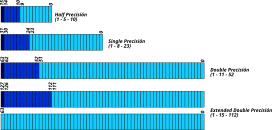
\includegraphics[width=\textwidth]{IEEE754-2008.pdf}
 \end{textblock*}
\end{frame}



\subsection{Precisión. Métricas}
\begin{frame}{Métricas de Precisión}
 \begin{textblock*}{\textwidth}(0.2cm,1.2cm)
  \begin{itemize} [<+(1)->]\justifying \parskip .2cm
   \item De acuerdo  a lo tratado hasta aquí, surgen algunos parámetros que pueden obrar como métricas al adoptar un determinado formato de representación para números en Punto Flotante en un computador.
   \item En el slide anterior se mostró la representación de tres números consecutivos: el número $1$, su inmediato anterior para esa precisión y el inmediato posterior.
   \item Esto implica que cualquier otro valor intermedio ubicado en uno u otro intervalo se redondea a $1$, o al número anterior o posterior de acuerdo con el criterio de redondeo establecido.
   \item  Además se ha tomado como ejemplo una representación con $p=24$.
  \end{itemize}
 \end{textblock*}
\end{frame}

\begin{frame}{Métricas de Precisión: Machine Epsilon}
 \begin{textblock*}{\textwidth}(0.2cm,1.2cm)
  \begin{itemize} [<+->]\justifying \parskip .2cm
   \item De acuerdo con la representación polinómica, el valor posterior a $1$ se representa de acuerdo con esta expresión:\\
   \centering $n = 1 + 1\cdot 2^{-23}$
   \item Por lo tanto la diferencia entre 1 y su inmediato posterior para su representación sin redondear es $2^{-23}$.
   \item Esta diferencia se denomina \textbf{\textit{machine epsilon}}, y representa la distancia entre $1$ y el mínimo número representable mayor que $1$.\\
   \centering $ \varepsilon = 2^{-(p-1)}$
   \item Por lo tanto, $\varepsilon$ resulta una métrica clara de la precisión que tiene un formato de representación.
  \end{itemize}
 \end{textblock*}
\end{frame}

\begin{frame}{Métricas de Precisión: \textit{ulp(x)}}
 \begin{textblock*}{\textwidth}(0.2cm,1.2cm)
  \begin{itemize} [<+(1)->]\justifying \parskip .2cm
   \item Otra propiedad que aporta información de interés para la representación de números en Punto Flotante es la denominada \textbf{\textit{ULP}}: referida como \textit{Unit in the Last Place} o \textit{Unit of Least Precision}~\cite{Overton2001}~\cite{Higham2002}.
   \item Se la define como el espacio entre dos números de Punto Flotante consecutivos capaces de ser representados sin redondeo. Esté relacionada con $\varepsilon$, pero representa algo mas general. Dado un número x, cuya representación en punto flotante resulta en $(m_{0}.m_{1}m_{2}...)\cdot 2^{e}$, se define mediante la siguiente expresión:\\
   \centering $ulp(x) = \frac {|m_{0}.m_{1}m_{2}... - \frac{x}{ 2^{-e}}|} {2^{(p-1)}}$
   \item Es la medida del error relativo entre un número \textit{x} y su representación en punto flotante para una precisión dada.
   \end{itemize}
 \end{textblock*}
\end{frame}

\begin{frame}{Métricas de Precisión: \textit{ulp(x)}}
 \begin{textblock*}{\textwidth}(0.2cm,1.2cm)
  \begin{itemize} [<+(1)->]\justifying \parskip .2cm
   \item Para entender su significado es conveniente trabajar con un modelo reducido conocido como \textbf{\textit{Toy Number System}} que consisten en tomar una repŕesentación mínima para observar a simple vista características que se van a mantener en el tiempo.
   \item Para ello consideremos un número representable con un \textit{significando} compuesto de un bit entero y dos fraccionarios y un \textit{exponente} de un bit.
   \item La expresión en este caso viene dada por:\\
        \centering $(m_{0}.m_{1}m_{2})_{2} \cdot 2^{e}, donde~ -1\leq e \leq 1, y~ e\in \mathbb{N}_{0}$
   \item Las posibles combinaciones del \textit{significando} son: $1.00_{2}, 1.01_{2}, 1.10_{2}, 1.11_{2}$.
   \item De acuerdo con esto y los posibles valores de \textit{exponente} detallados en la expresión anterior, la lista de valores que se obtienen de dicha expresión es:\\
   \only<7->{
    \hspace{1.8cm} \small [-3.5, -3, -2.5, -2, -1.75, -1.5, -1.25, -1, -0.875, -0.75, -0.625, -0.5,\\
    \hspace{1.8cm} \small  0, 0.5, 0.625, 0.75, 0.875, 1, 1.25, 1.5, 1.75, 2, 2.5, 3, 3.5].
    }
   \end{itemize}
 \end{textblock*}
\end{frame}

\begin{frame}{Modelo de representación: Toy Machine}
 \begin{textblock*}{\textwidth}(0.2cm,1.2cm)
  \begin{itemize} [<+->]\justifying \parskip .18cm
   \item Estos set de valores de Punto Flotante se representan gráficamente a continuación:\\
         \centering 
\includegraphics[width=\textwidth]{ToyMachine-2bit.pdf}\\
           \centering \textit{Toy Number System para \textbf{significando} de \SI{2}{\bit}}\\
         \centering 
\includegraphics[width=\textwidth]{ToyMachine.pdf}\\
           \centering \textit{Toy Number System  para \textbf{significando} de \SI{3}{\bit}}\\
   \item Toy Floating Point System Number, es un sistema discreto, en el que la cantidad de números en cada intervalo aumenta, junto con los bits del \textit{significando}.
   \item Visualmente es apreciable la diferencia entre las dos figuras anteriores.
   \item Una característica distintiva (y curiosa) es que el gap entre números no es constante sino que aumenta a medida que aumenta la magnitud de los números representados.
   \end{itemize}
 \end{textblock*}
\end{frame}

\begin{frame}{Modelo de representación: Toy Machine}
 \begin{textblock*}{\textwidth}(0.2cm,1.2cm)
  \begin{itemize} [<+->]\justifying \parskip .18cm
   \item Estos set de valores de Punto Flotante se representan gráficamente a continuación:\\
         \centering 
\includegraphics[width=\textwidth]{ToyMachine-2bit.pdf}\\
           \centering \textit{Toy Number System para \textbf{significando} de \SI{2}{\bit}}\\
         \centering 
\includegraphics[width=\textwidth]{ToyMachine.pdf}\\
           \centering \textit{Toy Number System  para \textbf{significando} de \SI{3}{\bit}}\\
   \item  En el modelo de \SI{2}{\bit} la distribución de los valores obtenidos no es uniforme. El gap entre valores próximos aumenta con el rango numérico que se represente.
   \item Si calculamos el \textbf{\textit{Machine Epsilon}} del sistema de números de precisión $p=3$, tenemos: $\varepsilon=2^{-(3-1)}=2^{-2}=0.25$.
   \item Observando el intervalo $[1.00,2.00]$ los valores posibles con este sistema de números son: $1, 1.25, 1.5, y 1.75$. Lo mismo ocurre para el intervalo $[-2.00, -1.00]$.
   \end{itemize}
 \end{textblock*}
\end{frame}

\begin{frame}{Métricas de Precisión de una Toy Machine}
 \begin{textblock*}{\textwidth}(0.2cm,1.2cm)
  \begin{itemize} [<+->]\justifying \parskip .18cm
   \item Estos set de valores de Punto Flotante se representan gráficamente a continuación:\\
         \centering 
\includegraphics[width=\textwidth]{ToyMachine-2bit.pdf}\\
           \centering \textit{Toy Number System para \textbf{significando} de \SI{2}{\bit}}\\
         \centering 
\includegraphics[width=\textwidth]{ToyMachine.pdf}\\
           \centering \textit{Toy Number System  para \textbf{significando} de \SI{3}{\bit}}\\
   \item Pero en los subsiguientes intervalos esta propiedad no se mantiene, de modo que solo en estos intervalos se verifica $ulp(x) =\varepsilon$.
   \item Ambas propiedades pueden verse mas claramente a medida que aumenta la precisión. En el modelo de \SI{3}{\bit} si bien aumenta un bit la precisión y la densidad de números por cada intervalo aumenta, se mantienen ambas propiedades.
   \item En el intervalo comprendido entre los números $[1.00, 2.00]$, puede verse que la distancia entre dos valores consecutivos coincide con el \textbf{\textit{Machine Epsilon}}.
   \end{itemize}
 \end{textblock*}
\end{frame}

\begin{frame}{Métricas de Precisión de una Toy Machine}
 \begin{textblock*}{\textwidth}(0.2cm,1.2cm)
  \begin{itemize} [<+->]\justifying \parskip .15cm
   \item La diferencia entre dos números consecutivos para un \textit{exponente} \textit{\textbf{e}} dado, está determinada por el bit menos significativo de la \textit{mantisa}.
   \item Otra forma de plantear la expresión de \textit{\textbf{ulp(x)}} para un número representado en punto flotante con precisión \textbf{\textit{p}}, es:

    \centering $ulp(x) = 0.00000 \dots 0001_{2}\cdot 2^{e}$

    \item $p-1$ bits en $0$, y el menos significativo en $1$, es la mínima diferencia del número x con el inmediato posterior, y  \textit{e}, el \textit{exponente} de la expresión normalizada de ambos.
    \item Desarrollando en potencias de 2 el número del segundo término se llega a:

    \centering $ulp(x) = 2^{-(p-1)}\cdot 2^{e}$

    \item Donde $2^{-(p-1)} = \varepsilon$, de modo de que esta expresión termina relacionando la precisión $\varepsilon$ y la exactitud \textbf{\textit{ulp(x)}} (ya que tiene que ver con el error de redondeo).

    \centering $ulp(x) = \varepsilon \cdot 2^{e}$

  \end{itemize}
 \end{textblock*}
\end{frame}

\begin{frame}{Métricas. Caso IEEE-754-2008}
 \begin{textblock*}{\textwidth}(0cm,1.2cm)
  \begin{itemize} [<+->]\justifying \parskip .15cm
   \item Los detalles acerca de cada formato son bien conocidos y existe numerosa bibliografía para consultar los pormenores.~\cite{Overton2001}. En~\cite{Sun2001} los autores realizan un análisis pormenorizado de los problemas de la no estandarización que derivaron en la norma IEE754 en 1985~\cite{Cowlishaw2003,Monieaux2008}.
   \item Half Precision, se introduce a propuesta de los desarrolladores de GPGPUs, ya que en un amplio conjunto de aplicaciones los requerimientos de rango comprenden intervalos relativamente pequeños y al tener un Épsilon $\varepsilon \approx 9.77 \cdot 10^{-4}$ puede satisfacer gran parte de los requerimientos de precisión por parte de sus aplicaciones.
   \item Para la misma cantidad de números se requiere la mitad de espacio de memoria, y se lee por cada transferencia el doble de datos, y la energía eléctrica consumida para su traslado hasta la GPGPU es mucho menor .
   \item En general la mayor parte de las aplicaciones trabajan con datos de tipo \textit{float}, ya que su $\varepsilon=2^{-23}$ permite efectuar cálculos con 7 dígitos decimales de precisión~\cite{Overton2001}, lo cual resulta mas que suficiente para una gran cantidad de problemas numéricos.
  \end{itemize}
 \end{textblock*}
\end{frame}

\begin{frame}{IEEE-754-2008}
 \begin{textblock*}{\textwidth}(0.3cm,1.2cm)%
  La Tabla muestra los valores de $\varepsilon$,  y \textbf{\textit{ulp}} para los diferentes formatos.
  \begin{table}[h]
   \begin{center}
    \begin{footnotesize}
     \begin{tabular}{||l|c|c|c|c|c||}
\hline\hline
\textbf{\textit{Tipo de Dato}} & Precisión &  Bias de  & $\varepsilon$ en base &  Decimales &\textbf{\textit{ulp(x)}}\\
                               &  [Bits]   & Exponente & 2 y en base 10 &  exactos   &\\
\hline\hline
Half Precision & 11 & 15 & $2^{-10} = 9.766\cdot10^-4$ & $\sim3.3$ & $3.2\cdot10^{1}$\\ \hline
Single Precision & 24 & 127 & $2^{-23} = 1.192\cdot10^{-7} $ & $\sim 7.2$ & $2.028240\cdot10^{31}$\\ \hline
Double Precision & 53 & 1023 & $2^{-52} = 2.220\cdot10^{-16} $ & $\sim15.9$ & $1.995840\cdot10^{292}$\\ \hline
x86 Extended Double& 65 & 16383 & $2^{-64} = 5.421\cdot10^{-20}$ & $\sim19.2$ & $6,449547×10^{4192}$\\ \hline
Quad & 113 & 16383 & $2^{-112} = 1.926\cdot10^{-34}$ & $\sim34.0$ & $1.1456698\cdot10^{4898}$\\
\hline\hline
     \end{tabular}
    \end{footnotesize}
   \end{center}
   \caption{Machine Epsilon y ulp(x) para los formatos IEEE754: Además en relación con el Machine Epsilon se puede calcular la cantidad de dígitos decimales exactos de cada precisión en formato decimal que es el que se termina presentando en las salidas de los programas}
   \label{tbl:epsilons}
  \end{table}
 \end{textblock*}
\end{frame}

\subsubsection{Representación en memoria}
\begin{frame}{Long Double}
 \begin{textblock*}{\textwidth}(0cm,1.2cm)
  \begin{itemize} [<+->]\justifying \parskip .15cm
   \item Este aspecto, que parecería apriori estar cerrado, en el caso del \textit{long double}, sin embargo, no es trivial.
   \item Los tipos \textit{float} y \textit{double} utilizados en el lenguaje C son bastante anteriores a la especificación IEEE-754, y podría decirse que tanto la norma como los diseños de hardware para implementar una FPU los han tomado como una referencia obligada.
   \item El tipo long double, por su parte, al no ser de uso tan frecuente en la mayor parte de las aplicaciones de uso corriente, no ha quedado debidamente cerrado, y su implementación terminó sujeta a cada arquitectura de hardware.
   \item Por tal motivo, los compiladores no lo tratan de manera uniforme.
   \item Incluso en una misma arquitectura como la x86 de Intel, que ha experimentado una larga evolución durante casi 5 décadas existen dos variantes, de acuerdo al modo en que trabaje el procesador:
  \end{itemize}
 \end{textblock*}
\end{frame}

\begin{frame}{Long Double}
 \begin{textblock*}{\textwidth}(0cm,1.2cm)
  \begin{description}
   \item [Modo IA-32:] Fundado por el procesador 80386 en 1984, es decir es previo a la especificación IEEE-754,  y vigente en la actualidad, un número especificado como long double utiliza \SI{12}{\byte} en memoria. Si bien es un modo legacy existen aun distribuciones de \SI{32}{\bit} (debian Linux es una de ellas para sistemas de gama baja), y en éstas una simple comprobación en lenguaje C mediante \texttt{sizeof (long double)}, verifica este tamaño que curiosamiente no coincide con los \SI{10}{\byte} de ancho de los registros de la FPU, que inspiraron el formato extended double de la especificación IEEE-754. En caso de requerirse que el dato tenga \SI{128}{\bit} se debe utilizar el flag \texttt{-128bit-long-double} del gcc para compilarlo.
   \item [Modo IA-32e:] Implementado en 2000 por AMD utiliza como tamaño default \SI{128}{\bit} para long double. El mismo código citado en el ítem anterior, pero ahora compilado en una instalación de 64 bits genera variables de 16 bytes por defecto.
  \end{description}
 \end{textblock*}
\end{frame}

\section{Arquitectura ARMv7. Punto flotante}
\subsection{Versiones de la extesión y registros}

\begin{frame}{Registros de Coprocesadores}
 \begin{textblock*}{\textwidth}(.3cm,1.2cm)
  \justifying La extensión VFP-v2, se basa en un co procesador que introduce un set de 32 registros de \SI{32}{\bit} para almacenar números en Punto Flotante simple precisión en formato IEEE-754.
 \end{textblock*}
 \begin{textblock*}{\textwidth}(.3cm,2.2cm)
  \centering \includegraphics[width=8cm]{VFP-Registers-layer1.pdf}
 \end{textblock*}
\end{frame}

\begin{frame}{Registros de las extensiones}
 \begin{textblock*}{\textwidth}(.3cm,1.2cm)
  \justifying Además VFP-v2 permite utilizar estos mismos registros de \SI{32}{\bit} para almacenar números en Punto Flotante doble precisión como 16 registros de \SI{64}{\bit} en formato IEEE-754.
 \end{textblock*}
 \begin{textblock*}{\textwidth}(.3cm,2.2cm)
  \centering \includegraphics[width=8cm]{VFP-Registers-layer2.pdf}
 \end{textblock*}
\end{frame}

\begin{frame}{Registros de las extensiones}
 \begin{textblock*}{\textwidth}(.3cm,1.2cm)
  \justifying Con la VFPv-3 se agregan otros 16 registros de \SI{64}{\bit}, para Punto Flotante doble precisión y para datos empaquetados en las Extensiones avanzadas SIMD (NEON).
 \end{textblock*}
 \begin{textblock*}{\textwidth}(.3cm,2.2cm)
  \centering \includegraphics[width=8cm]{VFP-Registers-layer3.pdf}
 \end{textblock*}
\end{frame}

\begin{frame}{Registros de las extensiones}
 \begin{textblock*}{\textwidth}(.3cm,1.2cm)
  \justifying Las Extensiones avanzadas SIMD (NEON) pueden trabajar con datos empaquetados de \SI{128}{\bit} agrupando los 32 registros de \SI{64}{\bit} en 16 registros de \SI{128}{\bit}.
 \end{textblock*}
 \begin{textblock*}{\textwidth}(.3cm,2.2cm)
  \centering \includegraphics[width=8cm]{VFP-Registers-layer4.pdf}
 \end{textblock*}
\end{frame}

\begin{frame}{References}
    \bibliographystyle{amsalpha}
    \bibliography{../../licar/bibliografia/Architecture/procarch}
\end{frame}
\end{document}
